\documentclass[10pt,a4paper]{scrartcl}
\usepackage[latin1]{inputenc}
\usepackage{amsmath}
\usepackage{amsfonts}
\usepackage{amssymb}
\usepackage{listings}
\usepackage{pdfpages}
\usepackage{url}
\usepackage[colorlinks=true,linkcolor=black]{hyperref}
\usepackage[T1]{fontenc}
\usepackage[ngerman]{babel}
\usepackage{enumitem}
\usepackage{blindtext} 
\begin{document}

\section{Lexikon}

\section{Allgemeines}
Aufz�hlungen der Aufgaben = 
\begin{enumerate} [leftmargin=1cm, label=\alph*)]
\item 
\item  
\item  
\end{enumerate}
Grafik einf�gen = \newline
\begin{center}
\begin{figure}[!htbp]
\fbox{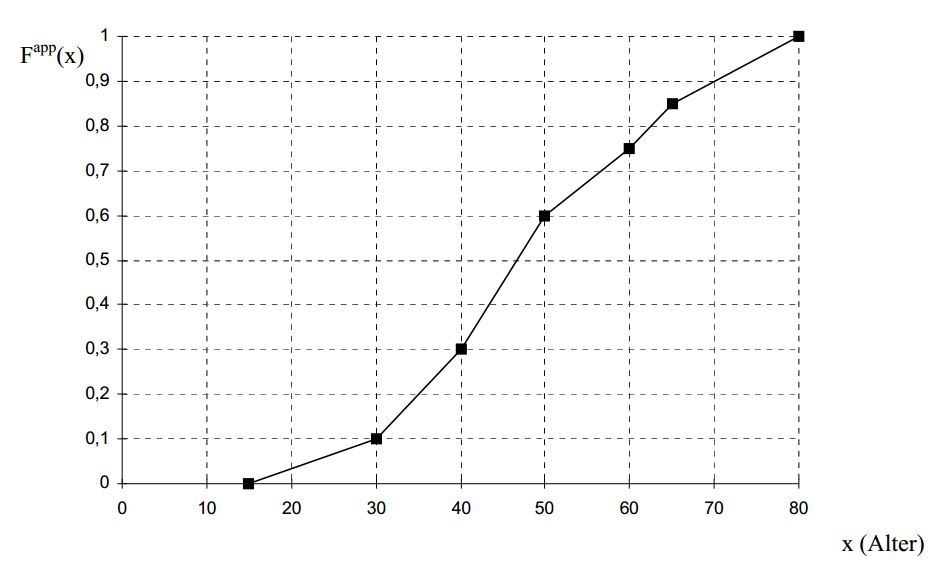
\includegraphics[width=0.9\textwidth,page=1]{./Grafiken/AB_1_11.jpg}} \caption{Erkl�rung}
\end{figure}
\end{center}

Summe = $\sum_{n=0}^N$
\newline
Index = $x_{0}$
\newline
Bruch = \( K=\dfrac{1}{11} \)
\newline
Tabelle
\newline
Horizonaler Strich mit = Siehe Code %hline
Vertikaler Strich mit = |
\newline
Reelle Zahlen = $\mathbb{R}$



\subsection{Griechische Symbole}
Omega = $\Omega$
\newline
Theta = 




\subsection{Mathematische Begriffe}
Grundraum Omega = $\Omega$
Wahrscheinlichkeitsraum = $(\Omega, \mathcal A , P )$
\newline
Wahrscheinlichkeit P(A) = $P (A)$
\newline
Mengenschreibweise = $\subset$  $\supset$  $\cap$  $\cup$
\newline
durchgestrichenes Gleichheitszeichen = $\neq$
\newline
Element von = $\in$ 
\newline
empirische Varianz = $\dfrac{1}{n}\sum_{i=1}^n(x_{i}-\overline{x})$
arithmetisches Mittle = $\overline{x}$


\end{document}